\documentclass{article}
\usepackage[utf8]{inputenc}
\usepackage{amsmath}
\usepackage{amsfonts}
\usepackage{graphicx}

\begin{document}

\title{Solution to Mock contest.}
\author{Prajit Adhikari}
\maketitle


\begin{enumerate}
  \item Let $f : \mathbb{R} \to \mathbb{R}$ be a function such that
$$f(f(x)) = x^2 - x + 1$$
for all real numbers $x$. Determine $f(0)$.\\
\textbf{Solution:}\\
Let, $P(x)$ be an assertion. Then, we have,
For $x=f(x)$,
$$f(f(f(x)))=f(x)^2-f(x)+1 \implies f(x^2-x+1)=f(x)^2-f(x)+1$$
For $x=1$, we get,
$$f(1)=f(1)^2-f(1)+1 \implies (f(1)-1)^2=0 \implies f(1)=1$$
Now, for $x=0$,we get,
$$f(1)=f(0)^2-f(0)+1 \implies f(0)(f(0)-1)=0 \implies f(0)=0,1$$
Now, checking back $f(0)=0,1$ in the original equation, we have,\\
For $f(0)=0$, $f(f(0))=0^2-0+1 \implies f(0)1$, which is absurd.\\
For $f(0)=1$, $f(f(0))=1 \implies f(1)=1$, which is true.\\
Hence, $\boxed{f(0)=1}$.
\newpage
  \item For a sequence $(a_n)_{n \geq 1}$ of real numbers it is known that $a_n = a_{n-1} + a_{n+2}$ for $n \geq 2$. What is the largest number of its consecutive elements that can all be positive?\\
\textbf{Solution:}\\
Let, us evaluate the expression for $n \to \infty$, we see that as
$$a_n=a_{n-1}+a_{n+2}$$
$$a_{n+1}=a_{n}+a_{n+3}$$
$$\vdots$$
Adding all the expression,we see that the $LHS$ will be zero, however $RHS$ will be sum i.e.
$$RHS= a_{n-1}+a_{n+2}+a_{n+3}+a_{n+4}+\hdots$$
which contradicts the fact that all numbers are positive.\\
Similarly, if we have more than $3$ equations then it is contradiction straight-forward, so,
$$ a_{n}=a_{n-1}+a_{n+2}$$
$$a_{n+1}=a_{n}+a_{n+3}$$
Adding two, we get,
$$ a_{n+1}=a_{n-1}+a_{n+2}+a_{n+3} \implies a_{n+1}=a_n+a_{n+3}$$
which is true. \\
Hence, the largest number of consecutive elements that can all be positive is $\boxed{5}$.

\newpage


\item  What is the smallest number of Bishops one can place on a $8 x 8$ Chess table so that all the cells of the table are attacked by at least one bishop? Provide an example.\\
\textbf{Solution:}\\
The bishops cover the diagonal of the of the chess board. A bishop can cover at most $15$ squares, so let's place two bishops at $d4$ and $d5$ position. Similarly, for placing other bishops now, if we put other two bishops adjacent to $d5$ and $d4$ at $d3$ and $d6$, we cover maximal number of squares with only 4 bishops, so we line up bishop on the $d-file$ or $e-file$ to get all squares covered with minimal number of bishops.
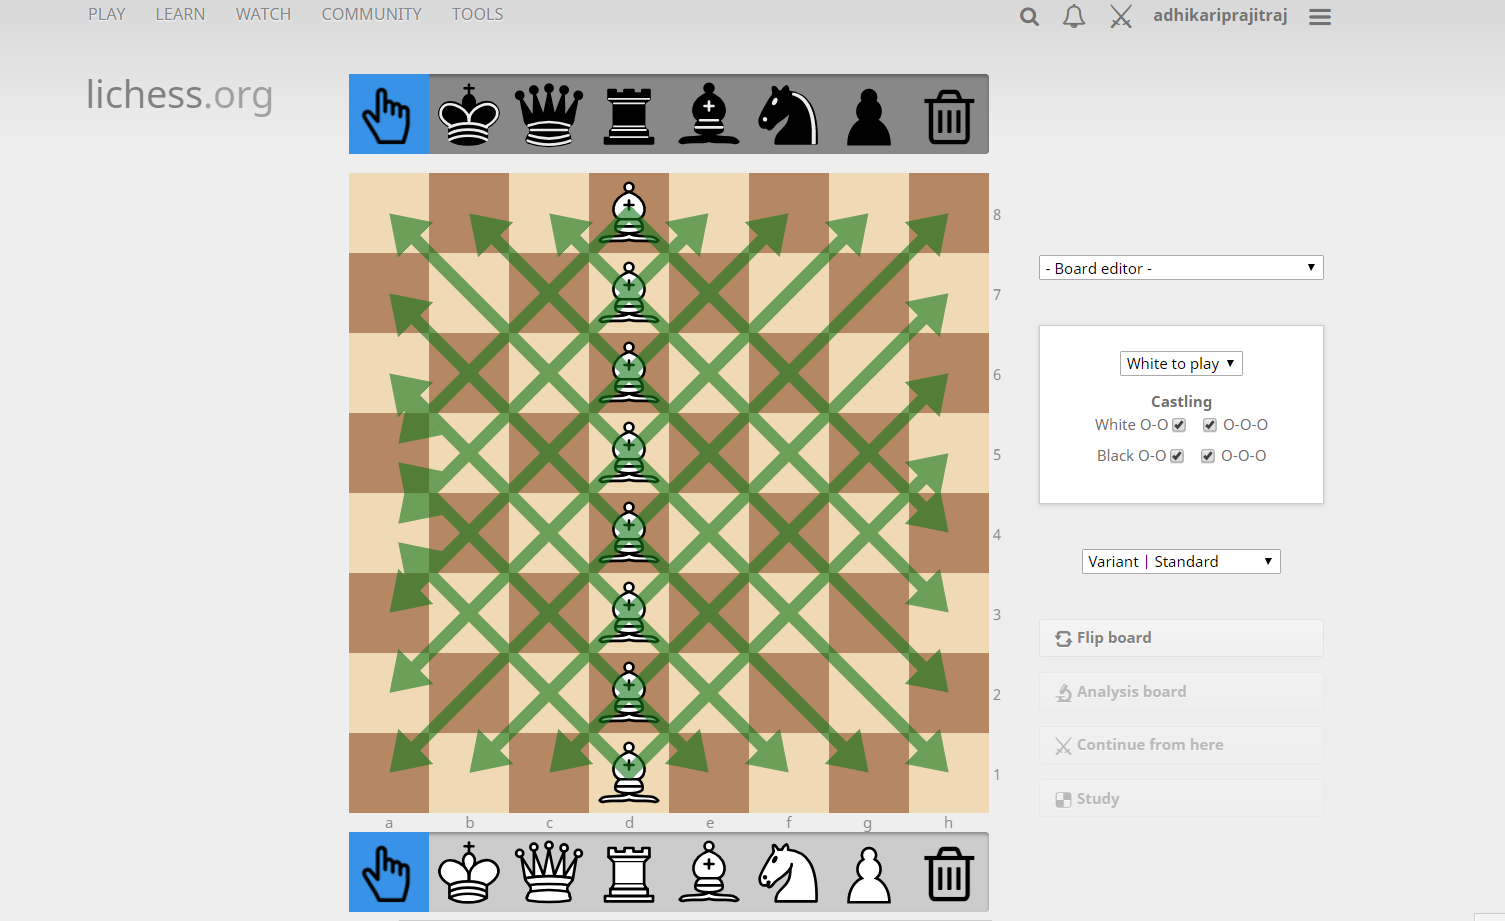
\includegraphics[width=\textwidth]{chess.PNG}

Proof: $7$ pieces doesn't work.\\
Let us invert the chess board $90^o$, then we see the diamond shaped chess board such that bishop act as rook. Now, this implies that $7$ rooks has to cover $64$ squares. If seven rooks are placed in the board, then each rooks cover at most $9$ squares without overlapping, so we get that, the maximal number of occupied square is $9*7=63$, so there will always be one square left, so $7$ bishops are insufficient.

Hence, the minimum number of bishops required is $\boxed{8}.$


\newpage

\item  A set of 8 problems was prepared for an examination. Each student was given 3 of them. No two students received more than one common problem. What is the largest possible number of students?\\
\textbf{Solution:}\\
There are $C(8,3)=56$ possible ways of giving problems to each students. However, there shouldn't be two same problems for two students.
Using Principle of Inclusion and Exclusion, we get that,
There are $2C(6,3)$ ways for the next student to select problem, and $2(4,3)$ ways for another student, then using PIE, we have, total unique problem set is given by:
$$56-2C(6,3)-2(4,3)=8$$
Hence, the largest possible number of student is $\boxed{8}$.

\newpage

\item  A sequence $a_1,a_2,a_3,...$ of non-negative integers is such that $a_{n+1}$ is the last digit of $a_n^n + a_{n-1}$ for all $n > 2$. Is it always true that for some $n_0$ the sequence $a_{n_0},a_{n_{0}+1},a_{n_{0}+2},...$ is periodic?\\
\textbf{Solution:}\\
We have that, by question,
$$a_n^n + a_{n-1} \equiv a_{n+1} \pmod{10}$$
Adding similar results we see that for any $k$, we have,
$$\sum_{i=n_0}^{k} a_{i}^i \equiv a_{k+1}+a_{k}-a_{n_0}-a_{n_0-1} \pmod{10}$$
which lasts forever. So, there must be $i,j$ such that $a_{i}=a_{j}$.








\newpage

\item  Find all finite sets of positive integers with at least two elements such that for any two numbers $a, b (a > b)$ belonging to the set, the number $\frac{b^2}{a-b}$ belongs to the set, too.\\
\textbf{Solution:}\\
Since, $a>b$, let $a=b+k$, then we have,
$k|b^2=m$. Let $S$ be a set of positive integers such that for $a,b \in S$, $m \in S$.Also, we have that, $a-b|b^2+a^2-b^2 \implies a-b|a^2 \implies a-b|a^2+b^2$.This implies that:
$$a-b|2ab \implies \frac{1}{2b}-\frac{1}{2a} \in \mathbb{Z^+}$$
$$\frac{1}{b}-\frac{1}{a} \in \mathbb{Z^+}$$
If $b=1$, then $a>1$, then $1-\frac{1}{a} \not \in \mathbb{Z^+}$.
Otherwise, $\frac{1}{b}-\frac{1}{a} <1$, so there do not exist such set.QED









\newpage

\item  The bisector of the angle A of a triangle ABC intersects BC in a point D and intersects the circumcircle of the triangle ABC in a point E. Let K,L,M and N be the midpoints of the segments AB,BD,CD and AC, respectively. Let P be the circumcenter of the triangle EKL, and Q be the circumcenter of the triangle EMN. Prove that $\angle PEQ = \angle BAC.$\\
\textbf{Solution:}\\
$$\angle AEC = \angle DEC$$
$$\angle BAE= \angle DAC=\angle BCE$$
$$ \Delta AEC \sim\Delta CED$$
Similarly,
$$\Delta ABE \sim\Delta BDE$$
Since these two triengles are similar, their median subtends same angle, so
$$\angle AEN= \angle MEC$$



\end{enumerate}


\end{document}
